\documentclass{article}
\usepackage{tikz}

\begin{document}

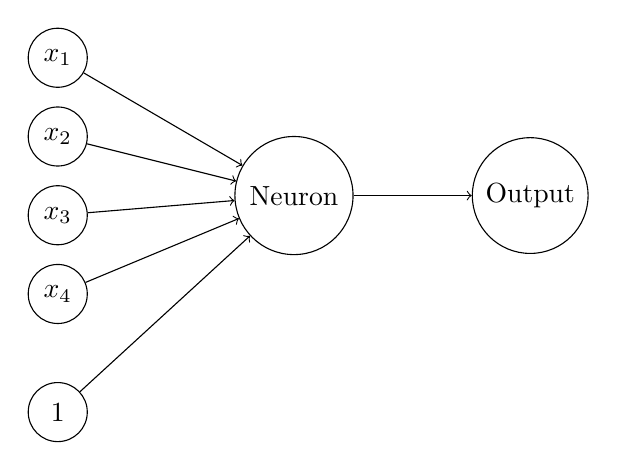
\begin{tikzpicture}
  % Input layer
  \foreach \i in {1,2,...,4}
    \node[circle, draw, minimum size=0.75cm] (input\i) at (0,-\i) {$x_\i$};

  % Bias unit
  \node[circle, draw, minimum size=0.75cm] (bias) at (0,-5.5) {1};

  % Neuron
  \node[circle, draw, minimum size=1.5cm] (neuron) at (3, -2.75) {Neuron};

  % Output node
  \node[circle, draw, minimum size=0.75cm] (output) at (6, -2.75) {Output};

  % Connect nodes
  \foreach \i in {1,2,...,4}
    \draw[->] (input\i) -- (neuron);
  \draw[->] (bias) -- (neuron);
  \draw[->] (neuron) -- (output);
\end{tikzpicture}

\end{document}
